\documentclass[lettersize,journal]{IEEEtran}
\usepackage{amsmath,amsfonts,amssymb,amsthm}
\usepackage{algorithmic}
\usepackage{array}
\usepackage[caption=false,font=normalsize,labelfont=sf,textfont=sf]{subfig}
\usepackage{textcomp}
\usepackage{stfloats}
\usepackage{url}
\usepackage{graphicx}
\usepackage{cite}
\usepackage{booktabs}
\usepackage{multirow}
\usepackage{tikz}
\usepackage{pgfplots}
\pgfplotsset{compat=1.17}
\usetikzlibrary{arrows.meta,positioning,decorations.pathreplacing}
\hyphenation{op-tical net-works semi-conduc-tor IEEE-Xplore}

% figure colours
\definecolor{c1}{HTML}{B4442F}
\definecolor{c2}{HTML}{2E7D8C}
\definecolor{c3}{HTML}{5B4B9B}
\definecolor{c4}{HTML}{B07D1E}
\definecolor{c5}{HTML}{2F6B45}

\newtheorem{theorem}{Theorem}
\newtheorem{assumption}{Assumption}

\newcommand{\Derr}{D_{\mathrm{err}}}
\newcommand{\Dagg}{D_{\mathrm{agg}}}
\newcommand{\Lamt}{\Lambda_{\mathrm{tot}}}
\newcommand{\Sb}{S_{\mathrm{b}}}

\begin{document}

\title{An Analytical Failure Criterion for Per-Site Dynamic Operating
Envelopes under Mobile Shared Flexible Loads}

\author{Author~One,~\IEEEmembership{Student Member,~IEEE,}
        and~Author~Two,~\IEEEmembership{Member,~IEEE}% <-this % stops a space
\thanks{The authors are with the Department of Electrical Engineering,
Institution, City, Country (e-mail: author@institution.edu).}% <-this % stops a space
\thanks{Manuscript received Month DD, YYYY; revised Month DD, YYYY.}}

\markboth{IEEE Transactions on Smart Grid,~Vol.~XX, No.~X, Month~YYYY}%
{Author \MakeLowercase{\textit{et al.}}: Analytical Failure Criterion for Per-Site Dynamic Operating Envelopes}

\maketitle

\begin{abstract}
Dynamic operating envelopes (DOEs) allocate a connection-specific,
per-interval power limit to each flexible customer and are secure by
construction in the linearised network model used to compute them. This paper
asks when that guarantee survives contact with a fleet of electric buses that
moves between charging hubs on the same feeder, and answers it with a
closed-form criterion. Two error terms are derived from the branch-flow
equations and shown to be additive at first order: the loss term the
linearised model omits, which is quadratic in power and carries the squared
shared-resistance fraction; and the drop caused by real dispatch moving within
a 15-minute envelope interval, which is linear in the intra-interval drift and
carries the shared-resistance fraction to the first power. Their sum,
normalised by the planning band, gives a single inequality computable from
topology and fleet parameters alone. Three supporting results are established:
corner certification of an envelope box remains exact at $N$ hubs; the loss
term admits an exact $N$-hub quadratic form whose coupling matrix is a Gram
matrix and hence positive semidefinite; and the mobility constant does not
enter the voltage criterion, so the mobile case reduces to the stationary
distributed-energy-resource condition. Validation uses 4\,760 static
allocations on 62 topologies and 48 full-day closed-loop simulations
(69\,120 minutes) on the IEEE 33-bus and 69-bus systems and two purpose-built
synthetic feeders, with every reported violation read from a
backward/forward-sweep AC solver rather than from the model the allocation was
optimised against. Adding the aggregation term raises per-minute recall from
$5.6\%$ to $82.2\%$ with no false positives; on 28 configurations held out from
threshold selection, precision and false-positive rate are preserved exactly
while recall is $0.852$--$1.000$. A decomposition shows the fleet drift
magnitude is invariant across every run and the entire coupling dependence is
the network sensitivity weight, matching measurement to three significant
figures on four topologies with no fitted quantity. A manipulation experiment
isolates the resistance profile of the hub's path as a driver of violation
incidence but not of the drift mechanism; the sign of the certified-slack
derivative on the 69-bus system remains unresolved and is scoped as future
work.
\end{abstract}

\begin{IEEEkeywords}
Dynamic operating envelopes, electric bus charging, distribution network
security, LinDistFlow, flexibility allocation, hosting capacity.
\end{IEEEkeywords}

\section*{Nomenclature}
\begin{tabular}{@{}ll@{}}
$u_i$ & Squared voltage magnitude at bus $i$ [p.u.]\\
$V_{\mathrm{ref}}$ & Substation voltage set point [p.u.]\\
$V_{\min}$ & Statutory lower voltage limit [p.u.]\\
$V_{\mathrm{plan}}$ & De-rated planning floor, $V_{\min}+\mathrm{band}$\\
$R_{ij},X_{ij}$ & Resistance/reactance shared by the root-to-$i$\\
 & and root-to-$j$ paths [p.u.]\\
$R_{m\ell}$ & Resistance shared by bus $m$ and branch $\ell$\\
$r_\ell$ & Resistance of branch $\ell$ [p.u.]\\
$\rho$ & Shared-resistance fraction $R_{AC}/R_{AA}$\\
$H$ & Number of charging hubs\\
$P_h,\bar P_h$ & Power and envelope cap of hub $h$ [kW]\\
$S_\ell,B_\ell$ & Total and base apparent flow in branch $\ell$\\
$L_k$ & Loss flowing through branch $k$\\
$\mathcal{P}(h)$ & Root-to-$h$ branch path\\
$C^{(m)},b^{(m)},c^{(m)}$ & Coefficients of the $N$-hub quadratic form\\
$\Sb$ & Power base [kVA]\\
$\Delta$ & Envelope interval length (15\,min)\\
$\delta p_j$ & Intra-interval injection deviation at bus $j$\\
$\gamma_j,\gamma_C$ & Intra-interval drift bound and its measured\\
 & value at hub C [kW]\\
$w_C$ & Voltage sensitivity to hub-C power\\
$\Derr,\Dagg$ & Loss and aggregation error terms [p.u.\ of $u$]\\
$\Lamt$ & Total failure index\\
$\tau$ & Mobility constant (travel plus dwell time)\\
$\alpha$ & Fairness exponent of the allocation objective\\
\end{tabular}

\section{Introduction}
\IEEEPARstart{D}{ynamic} operating envelopes are becoming the standard
mechanism by which distribution network service providers expose spare network
capacity to flexible customers \cite{petrou2021dol,liu2024robustdoe}. A DOE is,
by definition, connection-specific and per-interval: for each connection point
and each market interval the operator publishes an admissible power range, and
any dispatch inside the published set is guaranteed not to breach a network
constraint. The guarantee is delivered by solving an allocation problem over a
linearised network model, most often the LinDistFlow branch-flow relaxation
\cite{baran1989reconfig,farivar2013branchI,farivar2013branchII}, and it is exact \emph{within that
model}.

Electric bus fleets stress two of the assumptions behind that construction at
once. First, several opportunity-charging hubs commonly sit on the same feeder,
often on the same lateral, so their envelopes are not independent: the network
resource being allocated is shared. Second, and less obviously, the load itself
is mobile. A vehicle that charges at one hub departs and reappears at another
\cite{abdelwahed2020opportunity}, so charging demand is not a property of a
connection point but of a fleet whose spatial distribution changes on a
timescale comparable to the envelope interval.

The practical question is not whether a DOE is correct---it is, in its own
model---but under what conditions the residual between that model and the
physical network exceeds the safety margin the operator has retained. This
paper answers that question analytically, and the answer has two components
that have not previously been separated. One is the familiar linearisation
residual. The other, which dominates in closed loop, is a \emph{temporal
aggregation} residual: the envelope is computed once per interval against
interval-mean injections, while dispatch and exogenous load move within the
interval, and that movement propagates to a critical bus through the resistance
the hubs share.

\subsection{Contributions}
\begin{enumerate}
\item An exact $N$-hub expression for the loss term omitted by LinDistFlow,
obtained by an exchange of summation, and its expansion into a quadratic form
whose coupling matrix is a Gram matrix and therefore positive semidefinite
(Theorem~\ref{thm:nhub}). Corner certification of an envelope box is shown to
remain exact at $N$ hubs (Theorem~\ref{thm:corner}).
\item A first-order temporal-aggregation term in the same units and the same
certification framework, so the two are additive, together with a
planning-time bound expressed in drift rates and interval length
(Section~\ref{sec:agg}). The resulting single inequality \eqref{eq:lam} is
computable from topology, base-case flows and allocated caps without
simulation.
\item A demonstration that the mobility constant $\tau$ does not enter the
voltage criterion---the constraint is instantaneous and electrical---and that
the criterion reduces to the stationary single-site condition as
$\tau\!\to\!0$ (Section~\ref{sec:tau}).
\item A validation protocol in which no reported violation is read from the
model an allocation was optimised against, spanning 4\,760 static allocations
on 62 topologies and 48 full-day 1-minute closed-loop simulations on four
topologies, with two published test feeders held out from the derivation set.
\item A decomposition establishing that the entire coupling dependence of the
aggregation term is the network sensitivity weight rather than any change in
fleet behaviour, giving the closed form \eqref{eq:closedform}, and a
manipulation experiment that separates what controls the mechanism from what
controls violation incidence (Section~\ref{sec:mech}).
\end{enumerate}

\subsection{Organisation}
Section~\ref{sec:related} positions the work. Section~\ref{sec:model} states
the network and fleet model and the assumptions. Section~\ref{sec:derivation}
derives the two error terms and the criterion. Section~\ref{sec:method} gives
the validation protocol. Section~\ref{sec:results} reports results, including
the holdout and second-topology tests. Section~\ref{sec:mech} decomposes and
manipulates the mechanism. Section~\ref{sec:disc} generalises beyond bus
fleets, Section~\ref{sec:threats} states threats to validity, and
Section~\ref{sec:concl} concludes.

\section{Related Work}\label{sec:related}
Work on operating envelopes divides broadly into allocation methods---how to
share a feeder's headroom fairly and efficiently among connection
points---and deployment studies that report what happens when envelopes meet
real customers. The allocation literature is where the $\alpha$-fair family
used as the benchmark in this paper originates \cite{mo2000fair}, and it has
been developed for envelopes in both single-phase and unbalanced settings, with
explicit treatment of the equity of the resulting allocation
\cite{gerdroodbari2022pq,alam2024allocation}. Its defining commitment is that
limits are connection-specific rather than portfolio-wide
\cite{petrou2021dol}. Robust formulations extend the same construction to
hedge against forecast and data uncertainty \cite{liu2024robustdoe}.

Deployment trials have independently reported that envelope accuracy is
sensitive to how often the allocation is refreshed against updated forecasts,
with close-to-real-time envelopes outperforming day-ahead and intra-day ones
\cite{aemo_edge}. The present work explains why refresh cadence matters in a
way that is inseparable from network coupling: the error a stale envelope
admits reaches a critical bus through shared resistance, so cadence alone does
not determine whether a violation occurs.

%TODO: verify citation for the claim that electric-bus charging coordination
%      studies model the network either as a single aggregate constraint or via
%      full nonlinear OPF. Two or three recent surveys/papers should be cited
%      here; none could be verified from a primary record at the time of
%      writing, so the claim is stated without citation rather than supported
%      by an approximated reference.
Charging-coordination work for electric bus fleets has largely treated the
network either as a single aggregate constraint or through full nonlinear
optimal power flow; scheduling formulations in the transport literature
optimise charging against cost and grid impact without a per-connection network
limit \cite{abdelwahed2020opportunity}. The intermediate regime this paper
addresses---an operator publishing per-site limits, with the fleet optimising
inside them---is the one that matches how DOEs are actually deployed, and it is
where the two error terms below become visible.

\section{System Model and Assumptions}\label{sec:model}

\subsection{Network}
The feeder is radial with a single feed at bus~0 held at $V_{\mathrm{ref}}$.
Write $u_i=|V_i|^{2}$. Under the LinDistFlow relaxation
\cite{baran1989reconfig},
\begin{equation}\label{eq:lindist}
u_i \;=\; V_{\mathrm{ref}}^{2}-2\sum_{j}\bigl(R_{ij}p_j+X_{ij}q_j\bigr),
\end{equation}
where $R_{ij}$ is the total resistance of the branches common to the
root-to-$i$ and root-to-$j$ paths. Because $R_{ij}$ is a sum of positive branch
resistances, $R\succeq 0$ elementwise---the property that makes the corner
argument of Section~\ref{sec:corner} valid.

\begin{assumption}\label{as:radial}
Radial network, single feed held at $V_{\mathrm{ref}}$.
\end{assumption}
\begin{assumption}\label{as:lin}
Voltages follow \eqref{eq:lindist} at the planning stage.
\end{assumption}
\begin{assumption}\label{as:q}
Reactive injections are exogenous; hubs exercise no reactive control.
\end{assumption}
\begin{assumption}\label{as:loss}
Losses are small relative to flows, so a single loss-correction step suffices.
\end{assumption}

Assumption~\ref{as:lin} applies only at the planning stage; evaluation always
uses the exact AC solution, and Assumption~\ref{as:loss} is what licenses the
single correction step of \eqref{eq:derr}.
Fig.~\ref{fig:topology} shows the placement geometry used throughout: hub~A
sits at a lateral tip, hub~C is relocated along the path to it so that the
shared-resistance fraction $\rho=R_{AC}/R_{AA}$ is swept while the base case is
left unchanged, and hubs~B and~D sit on separate laterals.

\begin{figure}[!t]\centering
\resizebox{\columnwidth}{!}{% One-line diagram: coupling between two charging hubs on a radial feeder.
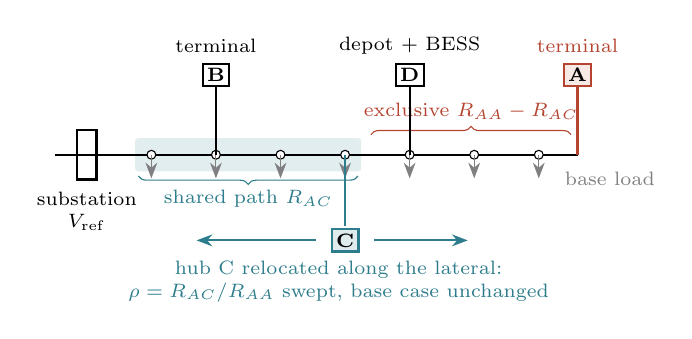
\begin{tikzpicture}[
  >={Stealth[length=2mm]},
  bus/.style={circle,draw,fill=white,inner sep=0pt,minimum size=3.2pt},
  lbl/.style={font=\scriptsize},
  hub/.style={rectangle,draw,thick,fill=white,inner sep=1.6pt,font=\scriptsize\bfseries},
  x=8.2mm,y=7.5mm]

% shared segment shading
\fill[c2!14,rounded corners=1pt] (0.75,-0.28) rectangle (4.25,0.28);

% trunk and buses
\draw[thick] (0,0) -- (7.6,0);
\foreach \x in {1,2,3,4,5,6,7} \node[bus] at (\x,0) {};
\foreach \x in {1,2,3,4,5,6,7} \draw[->,gray] (\x,0) -- ++(0,-0.40);
\node[lbl,gray] at (8.1,-0.40) {base load};

% substation
\draw[thick] (-0.15,-0.42) rectangle (0.15,0.42);
\draw[thick] (-0.5,0) -- (0,0);
\node[lbl,align=center] at (0,-0.95) {substation\\$V_{\mathrm{ref}}$};

% braces: shared (left, below) and exclusive (right, above)
\draw[decorate,decoration={brace,amplitude=3pt,mirror},c2] (0.8,-0.36) -- (4.2,-0.36);
\node[lbl,c2] at (2.5,-0.75) {shared path $R_{AC}$};
\draw[decorate,decoration={brace,amplitude=3pt},c1] (4.4,0.34) -- (7.5,0.34);
\node[lbl,c1] at (5.95,0.74) {exclusive $R_{AA}-R_{AC}$};

% hubs
\node[hub,fill=c1!12,draw=c1] (A) at (7.6,1.35) {A};
\draw[thick,c1] (7.6,0) -- (A);
\node[lbl,c1] at (7.6,1.85) {terminal};

\node[hub] (B) at (2,1.35) {B};
\draw[thick] (2,0) -- (B);
\node[lbl] at (2,1.85) {terminal};

\node[hub] (D) at (5,1.35) {D};
\draw[thick] (5,0) -- (D);
\node[lbl] at (5,1.85) {depot $+$ BESS};

% movable hub C
\node[hub,fill=c2!15,draw=c2] (C) at (4,-1.45) {C};
\draw[thick,c2] (4,0) -- (4,-1.2);
\draw[->,c2,thick] (4.45,-1.45) -- (5.9,-1.45);
\draw[->,c2,thick] (3.55,-1.45) -- (1.7,-1.45);
\node[lbl,c2,align=center] at (3.9,-2.15)
  {hub C relocated along the lateral:\\
   $\rho=R_{AC}/R_{AA}$ swept, base case unchanged};
\end{tikzpicture}
}
\caption{Coupling geometry. Hub~C is a bare en-route charging point with no site
load and no photovoltaics, so relocating it along hub~A's path changes $\rho$
without changing the base case.}
\label{fig:topology}
\end{figure}

\subsection{Envelope allocation}
For each interval the operator solves, over the hub caps
$P\in\mathbb{R}^{H}_{+}$,
\begin{equation}\label{eq:doe}
\max_{P}\;\textstyle\sum_h f_\alpha(P_h)
\quad\text{s.t.}\quad u(P)\ge V_{\mathrm{plan}}^{2},\;\; P\le \bar P^{\mathrm{PCC}},
\end{equation}
with $f_\alpha$ from the $\alpha$-fair family \cite{mo2000fair} ($\alpha=0$
efficiency, $\alpha=1$ proportional fairness, $\alpha\!\to\!\infty$ max-min).
Problem \eqref{eq:doe} is a \emph{joint} allocation: any combination inside the
resulting box is secure in the linear model. It is distinguished throughout
from the \emph{one-at-a-time} construction, in which each hub's headroom is
computed with the others held at base---a box that is not jointly feasible, and
that is included here only because a practitioner reading sensitivity factors
off a load-flow tool will produce it.

\subsection{Fleet and control architecture}
The lower level is a 1-minute model-predictive controller per hub, re-solved
every five minutes, that schedules charging inside the published envelope
subject to vehicle state of charge, bay availability and departure times.
Traction energy is exogenous: it is computed from longitudinal vehicle dynamics
over a synthetic urban duty cycle. The mobility constant $\tau$ denotes the
time for dispatch at one hub to affect state at another, i.e.\ travel plus
dwell. Fig.~\ref{fig:arch} shows the architecture and, in particular, the
separation between the allocation path and the evaluation path.

\begin{figure}[!t]\centering
\resizebox{0.98\columnwidth}{!}{% Control architecture and the evaluation discipline.
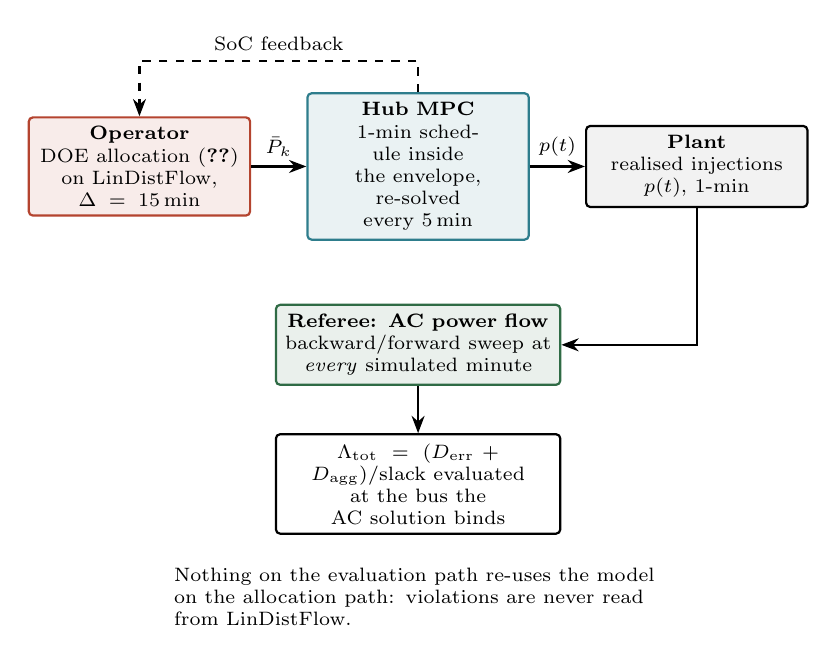
\begin{tikzpicture}[
  >={Stealth[length=2.2mm]},
  box/.style={rectangle,draw,thick,rounded corners=1.5pt,align=center,
              font=\scriptsize,minimum height=8.5mm,inner xsep=3pt},
  node distance=4mm,font=\scriptsize]

\node[box,fill=c1!10,draw=c1,text width=26mm] (doe)
  {\textbf{Operator}\\ DOE allocation \eqref{eq:doe}\\ on LinDistFlow, $\Delta=15$\,min};
\node[box,fill=c2!10,draw=c2,text width=26mm,right=7mm of doe] (mpc)
  {\textbf{Hub MPC}\\ 1-min schedule inside\\ the envelope, re-solved\\ every 5\,min};
\node[box,fill=black!5,text width=26mm,right=7mm of mpc] (plant)
  {\textbf{Plant}\\ realised injections\\ $p(t)$, 1-min};
\node[box,fill=c5!10,draw=c5,text width=34mm,below=8mm of mpc] (ac)
  {\textbf{Referee: AC power flow}\\ backward/forward sweep at\\ \emph{every} simulated minute};
\node[box,text width=34mm,below=6mm of ac] (crit)
  {$\Lamt=(\Derr+\Dagg)/\text{slack}$ evaluated\\ at the bus the AC solution binds};

\draw[->,thick] (doe) -- node[above,font=\scriptsize]{$\bar P_k$} (mpc);
\draw[->,thick] (mpc) -- node[above,font=\scriptsize]{$p(t)$} (plant);
\draw[->,thick] (plant.south) |- (ac.east);
\draw[->,thick] (ac) -- (crit);
\draw[->,dashed,thick] (mpc.north) -- ++(0,4mm) -| node[pos=0.25,above,font=\scriptsize]{SoC feedback} (doe.north);

\node[align=left,font=\scriptsize,below=3mm of crit,text width=62mm]
  {Nothing on the evaluation path re-uses the model on the allocation path:
   violations are never read from LinDistFlow.};
\end{tikzpicture}
}
\caption{Control architecture and the evaluation discipline. Every voltage
reported as a violation is computed by an AC power flow on the realised
1-minute injections, never by \eqref{eq:lindist}.}
\label{fig:arch}
\end{figure}

\section{Derivation}\label{sec:derivation}

\subsection{Corner certification at \texorpdfstring{$N$}{N} hubs}\label{sec:corner}
\begin{theorem}\label{thm:corner}
Under Assumptions~\ref{as:radial}--\ref{as:q}, $\min_i u_i$ over the box
$\prod_{h}[0,\bar P_h]$ is attained at the maximal corner $P=\bar P$, for any
number of hubs $H$.
\end{theorem}
\begin{proof}
From \eqref{eq:lindist}, $u_i(P)=u_i(0)-2\sum_h R_{ih}P_h$ with $R_{ih}\ge 0$,
so each $u_i$ is non-increasing in every coordinate of $P$. A function
non-increasing in each coordinate attains its minimum over a box at the maximal
corner; the pointwise minimum over $i$ of such functions inherits the property.
\end{proof}

Theorem~\ref{thm:corner} is what makes a single evaluation sufficient to
certify an entire envelope box, and nothing in the argument is pairwise---the
common restriction of coupling analyses to hub pairs is not required.

\subsection{Exact \texorpdfstring{$N$}{N}-hub form of the omitted loss term}
Exact DistFlow differs from \eqref{eq:lindist} in that branch flows carry the
losses generated downstream, plus a smaller $(r^{2}+x^{2})\ell$ term
\cite{baran1989capacitor}. Writing $\mathcal{P}(m)$ for the root-to-$m$ path
and $L_k$ for the loss flowing through branch $k$,
\begin{equation}\label{eq:lossdef}
\Derr(m)=2\!\!\sum_{k\in\mathcal{P}(m)}\!\! r_k L_k,
\qquad
L_k=\frac{1}{u}\sum_{\ell\succeq k} r_\ell S_\ell^{2}.
\end{equation}

\begin{theorem}\label{thm:nhub}
Exchanging the order of summation in \eqref{eq:lossdef} gives the exact,
non-pairwise identity
\begin{equation}\label{eq:derr}
\Derr(m)=\frac{2}{u}\sum_{\ell} r_\ell R_{m\ell} S_\ell^{2},
\end{equation}
where $R_{m\ell}$ is the resistance shared by bus $m$ and branch $\ell$.
Substituting $S_\ell=B_\ell+\sum_h \mathbf{1}[\ell\in\mathcal{P}(h)]P_h$ yields
\begin{equation}\label{eq:quad}
\Derr(m)=\frac{1}{u}\Bigl(P^{\!\top}C^{(m)}P+2\,b^{(m)\top}P+c^{(m)}\Bigr),
\end{equation}
\begin{equation}\label{eq:cmat}
C^{(m)}_{hh'}=\!\!\!\sum_{\ell\in\mathcal{P}(h)\cap\mathcal{P}(h')}\!\!\! r_\ell R_{m\ell},
\end{equation}
and $C^{(m)}$ is a Gram matrix of the vectors
$\bigl(\sqrt{r_\ell R_{m\ell}}\,\mathbf{1}[\ell\in\mathcal{P}(h)]\bigr)_\ell$,
hence positive semidefinite: $\Derr$ is convex in the allocated caps.
\end{theorem}
\begin{proof}
A branch $\ell$ contributes to every $k\in\mathcal{P}(m)$ upstream of it, and
the total resistance of those $k$ is by definition $R_{m\ell}$; exchanging the
two sums gives \eqref{eq:derr}. Expanding the square gives \eqref{eq:quad}, and
$C^{(m)}=G^{\!\top}G$ with $G_{\ell h}=\sqrt{r_\ell R_{m\ell}}\,
\mathbf{1}[\ell\in\mathcal{P}(h)]$ establishes positive semidefiniteness.
\end{proof}

For two hubs $A$ and $B$ with $\rho=R_{AB}/R_{AA}$, \eqref{eq:quad} collapses to
\begin{equation}\label{eq:pair}
\Derr(A)\approx\frac{2R_{AA}^{2}}{V_{\mathrm{ref}}^{2}}
\Bigl[\rho^{2}S_{\mathrm{sh}}^{2}+(1-\rho)^{2}S_{\mathrm{ex}}^{2}\Bigr],
\end{equation}
where $S_{\mathrm{sh}}$ carries the sum of both hubs' draws through the shared
segment and $S_{\mathrm{ex}}$ only hub $A$'s. Sharing therefore hurts
superlinearly, and hubs on separate laterals do not interact even at high
individual loading.

\subsection{Temporal aggregation}\label{sec:agg}
An envelope allocated once per interval of length $\Delta$ is planned against
interval-mean injections $\bar p$, while the plant realises $p(t)$
(Fig.~\ref{fig:timing}). Under \eqref{eq:lindist} the resulting additional drop
is exact and \emph{first} order:
\begin{equation}\label{eq:dagg}
\Dagg(m,t)=\frac{2}{\Sb}\sum_j\bigl[R_{mj}\,\delta p_j(t)+X_{mj}\,\delta q_j(t)\bigr]
\end{equation}
with $\delta p_j(t)=p_j(t)-\bar p_j$. If injection $j$ drifts at bounded rate
$|\dot p_j|\le\gamma_j$ then $\max_t|\delta p_j|\le\gamma_j\Delta/2$, giving the
planning-time bound
\begin{equation}\label{eq:daggbound}
\Dagg(m)\le\frac{\Delta}{2\Sb}\sum_j\bigl[R_{mj}\gamma_j+X_{mj}\gamma^{q}_j\bigr].
\end{equation}
Collapsed onto two hubs with $A$ at $m$,
$\Dagg(A)\le(\Delta/2\Sb)R_{AA}[\rho\gamma_{\mathrm{sh}}+(1-\rho)\gamma_{\mathrm{ex}}]$.
The structural contrast with \eqref{eq:pair} is the point: $\Derr$ is quadratic
in power and carries $\rho^{2}$, whereas $\Dagg$ is linear in drift and carries
$\rho^{1}$.

\begin{figure}[!t]\centering
\resizebox{0.96\columnwidth}{!}{% Why an interval-refreshed envelope admits an error the linear model cannot see.
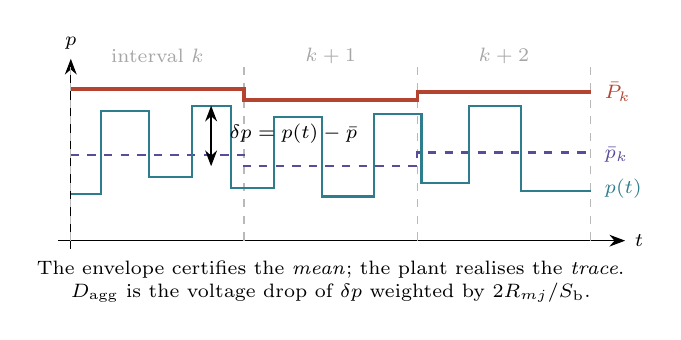
\begin{tikzpicture}[x=11mm,y=7mm,>={Stealth[length=2mm]},font=\scriptsize]
% axes
\draw[->] (-0.15,0) -- (6.4,0) node[right,font=\scriptsize] {$t$};
\draw[->] (0,-0.15) -- (0,3.3) node[above,font=\scriptsize] {$p$};

% interval boundaries
\foreach \x in {0,2,4,6} \draw[gray!55,dashed] (\x,0) -- (\x,3.15);
\node[gray!70] at (1,3.35) {interval $k$};
\node[gray!70] at (3,3.35) {$k+1$};
\node[gray!70] at (5,3.35) {$k+2$};

% envelope cap (staircase)
\draw[c1,very thick] (0,2.75) -- (2,2.75) -- (2,2.55) -- (4,2.55) -- (4,2.70) -- (6,2.70);
\node[c1,right] at (6.05,2.70) {$\bar P_k$};

% planning mean (staircase)
\draw[c3,thick,dashed] (0,1.55) -- (2,1.55) -- (2,1.35) -- (4,1.35) -- (4,1.60) -- (6,1.60);
\node[c3,right] at (6.05,1.55) {$\bar p_k$};

% realised 1-min dispatch
\draw[c2,thick]
  (0,0.85) -- (0.35,0.85) -- (0.35,2.35) -- (0.9,2.35) -- (0.9,1.15) -- (1.4,1.15)
  -- (1.4,2.45) -- (1.85,2.45) -- (1.85,0.95) -- (2.35,0.95) -- (2.35,2.25)
  -- (2.9,2.25) -- (2.9,0.80) -- (3.5,0.80) -- (3.5,2.30) -- (4.05,2.30)
  -- (4.05,1.05) -- (4.6,1.05) -- (4.6,2.45) -- (5.2,2.45) -- (5.2,0.90) -- (6,0.90);
\node[c2,right] at (6.05,0.95) {$p(t)$};

% the deviation that Dagg sees
\draw[<->,thick] (1.62,1.35) -- (1.62,2.45);
\node[align=left,anchor=west] at (1.72,1.95)
  {$\delta p=p(t)-\bar p$};
\node[align=center,font=\scriptsize] at (3.0,-0.75)
  {The envelope certifies the \emph{mean}; the plant realises the \emph{trace}.\\
   $\Dagg$ is the voltage drop of $\delta p$ weighted by $2R_{mj}/\Sb$.};
\end{tikzpicture}
}
\caption{Origin of the aggregation term. The envelope certifies the
interval-mean injection; the plant realises a 1-minute trace inside the
interval. $\Dagg$ is the voltage drop of that deviation, weighted by the
network sensitivity.}
\label{fig:timing}
\end{figure}

\subsection{The criterion}
The two terms are additive at first order, so
\begin{equation}\label{eq:lam}
\Lamt(m,t)=\frac{\Derr(m,t)+\Dagg(m,t)}
{u^{\mathrm{lin}}(m,\bar p(t))-V_{\min}^{2}}\;>\;1
\end{equation}
predicts an AC violation at bus $m$. The denominator is the certified slack:
the headroom the allocation's own linear model promised, which equals
$V_{\mathrm{plan}}^{2}-V_{\min}^{2}$ when the allocation binds. At a static
operating point $\Dagg\equiv 0$ and \eqref{eq:lam} reduces to the pure
linearisation criterion. Where the realised trace is unavailable at planning
time, the bound \eqref{eq:daggbound} replaces the second term of the
numerator. No quantity in either term is fitted.

\subsection{Where the mobility constant goes}\label{sec:tau}
$\tau$ does not appear in \eqref{eq:lam}, and this is a result rather than an
omission: the voltage constraint is instantaneous and electrical, so the
\emph{timing} of energy demand cannot enter it. $\tau$ governs energy
feasibility---whether the fleet meets its departures---and it enters the
voltage problem only through $\gamma$, by shaping how sharply hub power steps
within an interval. As $\tau\!\to\!0$ the hubs merge into one connection point:
$R_{AB}\!\to\!R_{AA}$, $\rho\!\to\!1$, $S_{\mathrm{ex}}\!\to\!0$, and
\eqref{eq:lam} collapses to the stationary single-site condition
\begin{equation}\label{eq:stationary}
\frac{2R^{2}S^{2}}{V_{\mathrm{ref}}^{2}}+\frac{\Delta R\gamma}{\Sb}\;>\;\mathrm{band}.
\end{equation}
Condition \eqref{eq:stationary} is the ordinary stationary envelope safety
condition, so the mobile case is a generalisation of the stationary
distributed-energy-resource case, not a departure from it.

\section{Validation Protocol}\label{sec:method}
Two regimes are used. \emph{Static}: an allocation is computed at one operating
point, all hubs are pushed to their caps simultaneously
(Theorem~\ref{thm:corner}), and the corner is evaluated by AC sweep.
\emph{Closed loop}: a full day is simulated at 1-minute resolution with the
envelope refreshed every 15 minutes and the hub MPC re-solved every 5 minutes;
$\Lamt$ is evaluated at every minute at the bus the AC solution says binds.

\emph{Derivation set.} 60 synthetic radial feeders with randomised branching
and MV-plausible impedances, crossed with five $\rho$ targets, three baseline
margins and three planning bands.

\emph{Held-out feeders.} The IEEE 33-bus and IEEE 69-bus systems, neither used
in deriving or tuning anything. The 69-bus data are parsed directly from
MATPOWER's \texttt{case69.m} \cite{zimmerman2011matpower}, whose header cites
Baran and Wu \cite{baran1989capacitor} and Das \cite{das2008capacitors}; the
parser is validated by reproducing the published base case, a minimum voltage
of $0.9092$~p.u.\ at bus~65, and $0.9131$~p.u.\ at bus~18 for the 33-bus
system, both at a $1.0$~p.u.\ slack.

\emph{Closed-loop sets.} Four topologies, 48 full-day runs, 69\,120 simulated
minutes. Sets~A and~B are the IEEE 33-bus system with hub~C moved along a
lateral through seven placements each; set~B uses five placements never seen
when the operating threshold was chosen, plus two at a larger fleet. Set~C is
the IEEE 69-bus system at a matched base-case minimum voltage ($0.9567$ against
$0.9572$). Sets~D and~E are two purpose-built synthetic feeders used for the
manipulation experiment of Section~\ref{sec:manip}.

\section{Results}\label{sec:results}

\subsection{Static allocations}
Table~\ref{tab:static} reports the static regime. One-at-a-time allocation
over-allocates by a median factor of exactly $2.000$ for two hubs, matching the
$N$-hub derivation, and violates in $98.4\%$ of synthetic and $53$--$100\%$ of
published-feeder configurations. Jointly certified allocation with any band
$\ge 0.005$~p.u.\ violates in $0$ of $1350$ synthetic, $0$ of $25$ IEEE 33-bus
and $0$ of $25$ IEEE 69-bus cases. The static classification is therefore
degenerate---there are no positives to discriminate---so no receiver operating
characteristic is reported and no threshold is fitted at a static point. On the
one non-degenerate column (joint, zero band) the index exceeds unity for all
797 violations with 13 false positives.

\begin{table}[!t]
\renewcommand{\arraystretch}{1.15}
\caption{Static Regime. Depths in p.u.}
\label{tab:static}
\centering\footnotesize
\begin{tabular}{@{}llrrrr@{}}
\toprule
Set & Mode & Band & $n$ & Violated & Med.\ depth\\
\midrule
Synthetic & one-at-a-time & 0.000 & 810 & 98.4\% & 0.0186\\
Synthetic & one-at-a-time & 0.005 & 810 & 98.4\% & 0.0111\\
Synthetic & one-at-a-time & 0.010 & 810 & 57.2\% & 0.0019\\
Synthetic & joint & 0.000 & 810 & 98.4\% & 0.0035\\
Synthetic & joint & 0.005 & 810 & 0.0\% & ---\\
Synthetic & joint & 0.010 & 540 & 0.0\% & ---\\
\midrule
IEEE 33 & one-at-a-time & 0.005 & 15 & 100\% & 0.0107\\
IEEE 33 & joint & 0.005 & 15 & 0.0\% & ---\\
IEEE 69 & one-at-a-time & 0.005 & 15 & 53.3\% & 0.0127\\
IEEE 69 & joint & 0.005 & 15 & 0.0\% & ---\\
\bottomrule
\end{tabular}
\end{table}

Fig.~\ref{fig:boundary} plots the resulting failure boundary: the band a
planner must hold at a static operating point. Joint allocation requires
$0.0055$--$0.0062$~p.u., nearly flat in $\rho$; one-at-a-time allocation
requires $0.019$--$0.031$~p.u.\ and rising.

\begin{figure}[!t]\centering
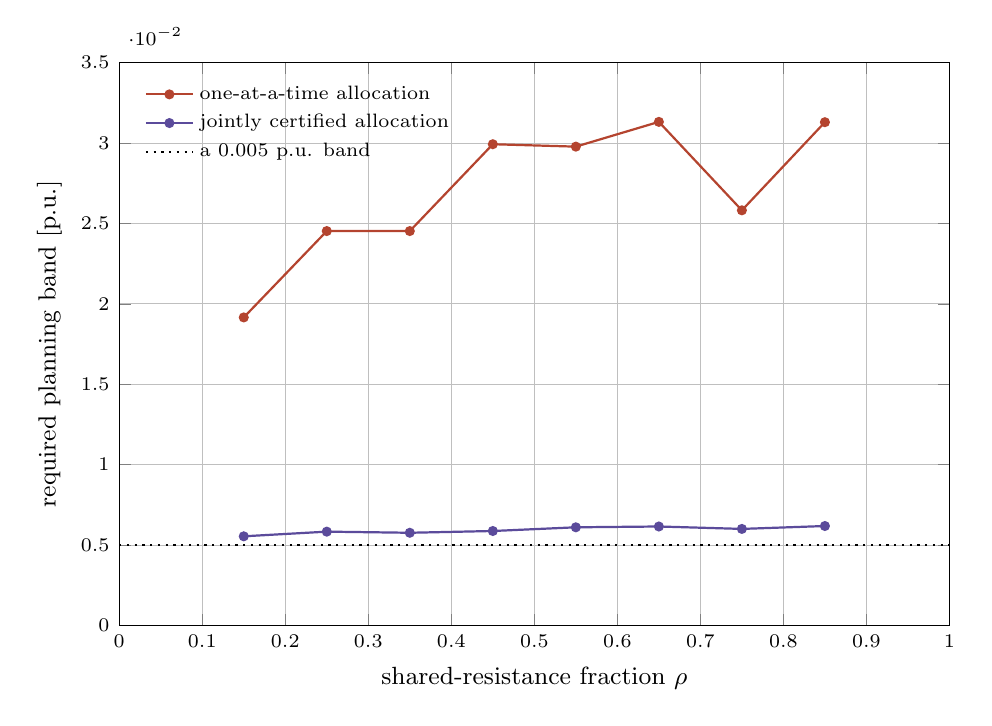
\begin{tikzpicture}
\begin{axis}[width=\columnwidth,height=0.72\columnwidth,
  xlabel={shared-resistance fraction $\rho$},
  ylabel={required planning band [p.u.]},
  xmin=0,xmax=1,ymin=0,ymax=0.035,grid=major,
  legend style={font=\scriptsize,at={(0.02,0.98)},anchor=north west,draw=none,fill=none},
  legend cell align=left,tick label style={font=\scriptsize},label style={font=\small}]
\addplot[c1,mark=*,mark size=1.4,thick] coordinates {(0.1500,0.01916) (0.2500,0.02453) (0.3500,0.02453) (0.4500,0.02993) (0.5500,0.02978) (0.6500,0.03132) (0.7500,0.02582) (0.8500,0.03130)};
\addlegendentry{one-at-a-time allocation}
\addplot[c3,mark=*,mark size=1.4,thick] coordinates {(0.1500,0.00555) (0.2500,0.00584) (0.3500,0.00577) (0.4500,0.00588) (0.5500,0.00611) (0.6500,0.00616) (0.7500,0.00601) (0.8500,0.00619)};
\addlegendentry{jointly certified allocation}
\addplot[black,dotted,thick] coordinates {(0,0.005) (1,0.005)};
\addlegendentry{a 0.005 p.u. band}
\end{axis}
\end{tikzpicture}

\caption{Static failure boundary on the $(\rho,\text{margin})$ plane. Curves
are the band required to stay secure; allocations below a curve are predicted
to violate. These are static bands only---the closed loop adds up to a further
$0.014$~p.u.}
\label{fig:boundary}
\end{figure}

\subsection{\texorpdfstring{$N$}{N}-hub check}
Forty configurations were tested: the four-hub IEEE 33-bus case study and
$H=2,3,4,5$ on IEEE 69-bus, at three baseline margins and three bands. The
quadratic form \eqref{eq:quad} agrees with an independent loss-propagation
computation to a maximum relative difference of $5\times10^{-16}$ at every $H$;
$C^{(m)}$ in \eqref{eq:cmat} is positive semidefinite in every case; and corner
certification is never violated by the AC solver once a band exists.

\subsection{Closed loop}\label{sec:closed}
Table~\ref{tab:closed} reports the closed-loop regime and
Fig.~\ref{fig:closedloop} the violation counts. Adding $\Dagg$ raises
per-minute recall from $5.6\%$ to $82.2\%$ at a $0.005$ band and from $0\%$ to
$79.6\%$ at $0.010$, with zero false positives in all 69\,120 simulated
minutes.

Three placements at low coupling are the control that rules out a
refresh-cadence-only explanation: at $\rho\le 0.276$ the same cadence, fleet
and drift magnitude produce \emph{zero} violations, because the deviation lands
at a bus with abundant certified slack. Cadence is necessary but not
sufficient; coupling is what converts it into a violation.

\begin{table}[!t]
\renewcommand{\arraystretch}{1.1}
\caption{Closed Loop, Band 0.005 p.u. Set A is the Threshold-Selection Set;
Sets B and C Were Not Used to Choose Any Threshold}
\label{tab:closed}
\centering\footnotesize
\begin{tabular}{@{}llrrrrr@{}}
\toprule
Set & $\rho$ & Viol.\ min & $\Derr$ & $\Dagg$ p95 & slack p5 & TP/FN\\
\midrule
\multirow{7}{*}{A}
 & 0.008 & 0  & 0.00197 & 0.01046 & 0.01200 & ---\\
 & 0.086 & 0  & 0.00192 & 0.00655 & 0.01167 & ---\\
 & 0.276 & 0  & 0.00159 & 0.00398 & 0.01042 & ---\\
 & 0.515 & 51 & 0.00141 & 0.00979 & 0.00802 & 36/15\\
 & 0.696 & 69 & 0.00139 & 0.01292 & 0.00639 & 57/12\\
 & 0.817 & 79 & 0.00142 & 0.01357 & 0.00539 & 67/12\\
 & 0.934 & 87 & 0.00142 & 0.01398 & 0.00524 & 75/12\\
\midrule
\multirow{7}{*}{B}
 & 0.194 & 0   & 0.00176 & 0.00415 & 0.01131 & ---\\
 & 0.369 & 33  & 0.00143 & 0.00503 & 0.00942 & 0/33\\
 & 0.463 & 46  & 0.00141 & 0.00813 & 0.00850 & 24/22\\
 & 0.515$^{\dagger}$ & 65 & 0.00161 & 0.00931 & 0.00574 & 46/19\\
 & 0.647 & 66  & 0.00140 & 0.01218 & 0.00682 & 51/15\\
 & 0.750 & 73  & 0.00142 & 0.01318 & 0.00595 & 62/11\\
 & 0.934$^{\dagger}$ & 109 & 0.00179 & 0.00969 & 0.00159 & 96/13\\
\midrule
\multirow{6}{*}{C}
 & 0.000 & 0  & 0.00242 & 0.00910 & 0.00953 & ---\\
 & 0.250 & 0  & 0.00244 & 0.00872 & 0.01573 & ---\\
 & 0.465 & 0  & 0.00257 & 0.00881 & 0.01414 & ---\\
 & 0.611 & 0  & 0.00271 & 0.00756 & 0.01328 & ---\\
 & 0.731 & 27 & 0.00274 & 0.00737 & 0.01259 & 0/27\\
 & 0.860 & 42 & 0.00272 & 0.00782 & 0.01185 & 27/15\\
\bottomrule
\end{tabular}\\[2pt]
\raggedright\footnotesize A, B: IEEE 33-bus; C: IEEE 69-bus. TP/FN at
$\Lamt>1$. $^{\dagger}$20-vehicle fleet; all other rows 16 vehicles.
\end{table}

\begin{figure}[!t]\centering
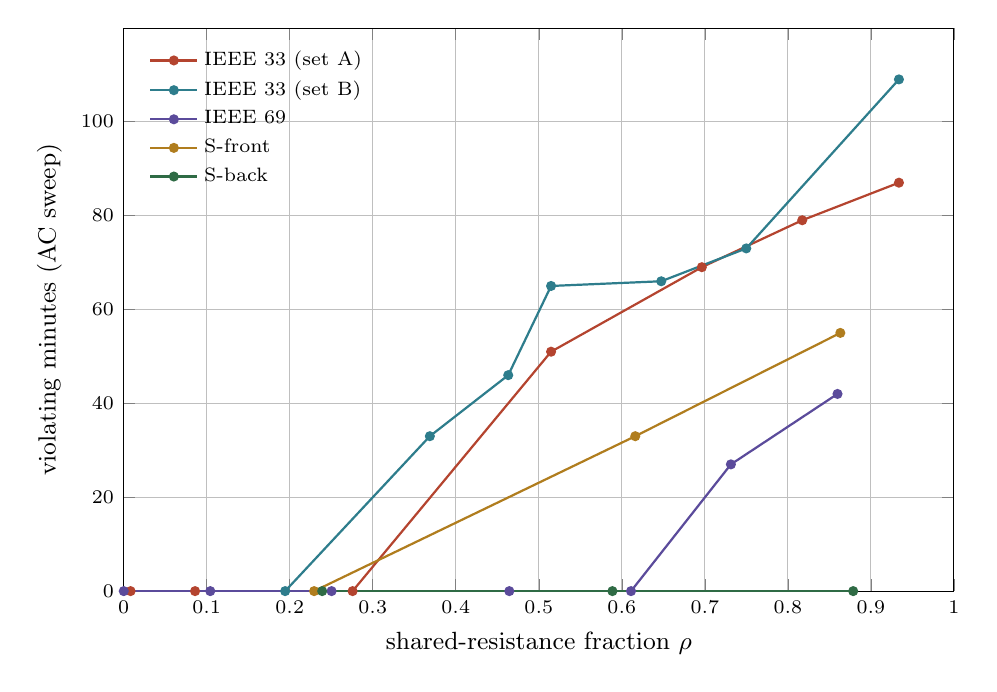
\begin{tikzpicture}
\begin{axis}[width=\columnwidth,height=0.72\columnwidth,
  xlabel={shared-resistance fraction $\rho$},
  ylabel={violating minutes (AC sweep)},
  xmin=0,xmax=1,ymin=0,grid=major,
  legend style={font=\scriptsize,at={(0.02,0.98)},anchor=north west,draw=none,fill=none},
  legend cell align=left,tick label style={font=\scriptsize},label style={font=\small}]
\addplot[c1,mark=*,mark size=1.4,thick] coordinates {(0.0083,0) (0.0860,0) (0.2757,0) (0.5148,51) (0.6964,69) (0.8173,79) (0.9338,87)};
\addlegendentry{IEEE 33 (set A)}
\addplot[c2,mark=*,mark size=1.4,thick] coordinates {(0.1945,0) (0.3688,33) (0.4632,46) (0.5148,65) (0.6475,66) (0.7499,73) (0.9338,109)};
\addlegendentry{IEEE 33 (set B)}
\addplot[c3,mark=*,mark size=1.4,thick] coordinates {(0.0001,0) (0.1043,0) (0.2504,0) (0.4645,0) (0.6111,0) (0.7314,27) (0.8598,42)};
\addlegendentry{IEEE 69}
\addplot[c4,mark=*,mark size=1.4,thick] coordinates {(0.2294,0) (0.6162,33) (0.8632,55)};
\addlegendentry{S-front}
\addplot[c5,mark=*,mark size=1.4,thick] coordinates {(0.2391,0) (0.5887,0) (0.8787,0)};
\addlegendentry{S-back}
\end{axis}
\end{tikzpicture}

\caption{Violating minutes against $\rho$, band 0.005~p.u., all closed-loop
sets. The monotone rise and a violation-free low-coupling regime replicate on
every topology; the coupling threshold at which violations begin differs
($\rho\approx0.4$ on IEEE 33, $\rho\approx0.7$ on IEEE 69), consistent with the
latter's larger certified slack.}
\label{fig:closedloop}
\end{figure}

\subsection{Threshold on a genuine holdout}\label{sec:holdout}
The practical trigger $\Lamt>0.85$ was chosen on set~A. Applied unchanged to
the 28 runs of sets~B and~C, it preserves precision and false-positive rate
exactly and loses recall (Table~\ref{tab:holdout}). The value was not adjusted
after seeing the holdout. It is therefore reported as bounded rather than
universal: validated for $\rho\in[0.00,0.93]$, bands $0.005$ and $0.010$~p.u.,
baseline margin $\approx 0.956$~p.u., 15-minute refresh with 5-minute MPC
re-solve, fleets of 16 and 20 vehicles, on two radial feeders. The derivation's
own threshold remains $\Lamt>1$.

\begin{table}[!t]
\renewcommand{\arraystretch}{1.15}
\caption{Threshold Generalisation. Holdout Rows Use $0.85$ Exactly as Selected
on Set A, With No Retuning}
\label{tab:holdout}
\centering\footnotesize
\begin{tabular}{@{}llrrrr@{}}
\toprule
Set & Rule & Band & Recall & Precision & FPR\\
\midrule
A (selection) & $\Lamt>1$    & 0.005 & 0.822 & 1.000 & 0.00000\\
A (selection) & $\Lamt>0.85$ & 0.005 & 0.955 & 1.000 & 0.00000\\
A (selection) & $\Lamt>0.85$ & 0.010 & 0.941 & 1.000 & 0.00000\\
\midrule
B (holdout)   & $\Lamt>1$    & 0.005 & 0.712 & 1.000 & 0.00000\\
B (holdout)   & $\Lamt>0.85$ & 0.005 & 0.852 & 1.000 & 0.00000\\
B (holdout)   & $\Lamt>0.85$ & 0.010 & 0.856 & 1.000 & 0.00000\\
C (holdout)   & $\Lamt>1$    & 0.005 & 0.391 & 1.000 & 0.00000\\
C (holdout)   & $\Lamt>0.85$ & 0.005 & 1.000 & 1.000 & 0.00000\\
C (holdout)   & $\Lamt>0.85$ & 0.010 & 1.000 & 1.000 & 0.00000\\
\bottomrule
\end{tabular}
\end{table}

The recall loss is localised and explainable. The holdout placement at
$\rho=0.369$ sits at the lower edge of the violating regime, where violation
depths are $0.0008$--$0.0010$~p.u.---the same size as the first-order model's
own reconstruction residual, whose mean absolute error is
$1.3\times10^{-3}$ in $u$ on IEEE 33 and $8.8\times10^{-4}$ on IEEE 69. The
index resolves violations deeper than its residual and cannot resolve shallower
ones.

\section{What Drives the Coupling Dependence}\label{sec:mech}

\subsection{Decomposition}
Measured as the 95th percentile of the \emph{aggregate} $\Dagg$, IEEE~33 shows
a rise with $\rho$ and IEEE~69 does not (Fig.~\ref{fig:split}). That statistic
is misleading, and it is the statistic behind the apparent disagreement between
sets in Section~\ref{sec:closed}: the aggregate mixes the hub's own drift term with a background
from every other bus's deviation, and a percentile of a signed sum is not the
sum of its parts. Splitting the hub's contribution into how much the fleet
drifts and how much the network weights that drift,
\begin{equation}\label{eq:split}
\Dagg^{C}(m)=w_C\,\gamma_C,\qquad w_C=\frac{2R_{mC}}{\Sb}=\frac{2R_{mm}}{\Sb}\rho,
\end{equation}
resolves it. Both factors in \eqref{eq:split} were measured separately at every minute of all 48
closed-loop runs. The drift magnitude is invariant: $\gamma_C$ is
$90.0$--$91.1$~kW (p95) in every run, at every $\rho$, on every feeder, at both
fleet sizes and both bands. It is a property of the charger---$90$~kW is
$0.6\times$ hub~C's single $150$~kW bay---not of the network. The entire
$\rho$-dependence is $w_C$, which is proportional to $\rho$ by construction:
the correlation between $\rho$ and $w_C$ is $+1.000$ on every set. Hence
\begin{equation}\label{eq:closedform}
\Dagg^{C}(m)=\frac{2R_{mm}\gamma_C}{\Sb}\,\rho,
\end{equation}
which contains no fitted quantity. Table~\ref{tab:collapse} and
Fig.~\ref{fig:collapse} compare it with measurement.

\begin{table}[!t]
\renewcommand{\arraystretch}{1.15}
\caption{Slope of the Hub Drift Term Against $\rho$ Versus the Closed Form
\eqref{eq:closedform}. Band 0.005 p.u.}
\label{tab:collapse}
\centering\footnotesize
\begin{tabular}{@{}lrrrrr@{}}
\toprule
Set & $R_{mm}$ & $\gamma_C$ & observed & $2R_{mm}\gamma_C/\Sb$ & ratio\\
\midrule
A: IEEE 33 & 0.0690 & 90.1 & 0.01243 & 0.01243 & 1.000\\
B: IEEE 33, 16 veh. & 0.0690 & 90.0 & 0.01243 & 0.01242 & 1.000\\
C: IEEE 69 & 0.0463 & 90.2 & 0.00838 & 0.00836 & 1.003\\
D: synthetic, front & 0.0474 & 90.1 & 0.00854 & 0.00854 & 1.000\\
E: synthetic, back & 0.0474 & 90.1 & 0.00854 & 0.00854 & 1.000\\
\midrule
B incl.\ 20-veh.\ runs & 0.0690 & 90.0 & 0.01002 & 0.01242 & 0.807\\
\bottomrule
\end{tabular}\\[2pt]
\raggedright\footnotesize $R_{mm}$ in p.u., $\gamma_C$ in kW, slopes in p.u.\
of $u$ per unit $\rho$.
\end{table}

\begin{figure}[!t]\centering
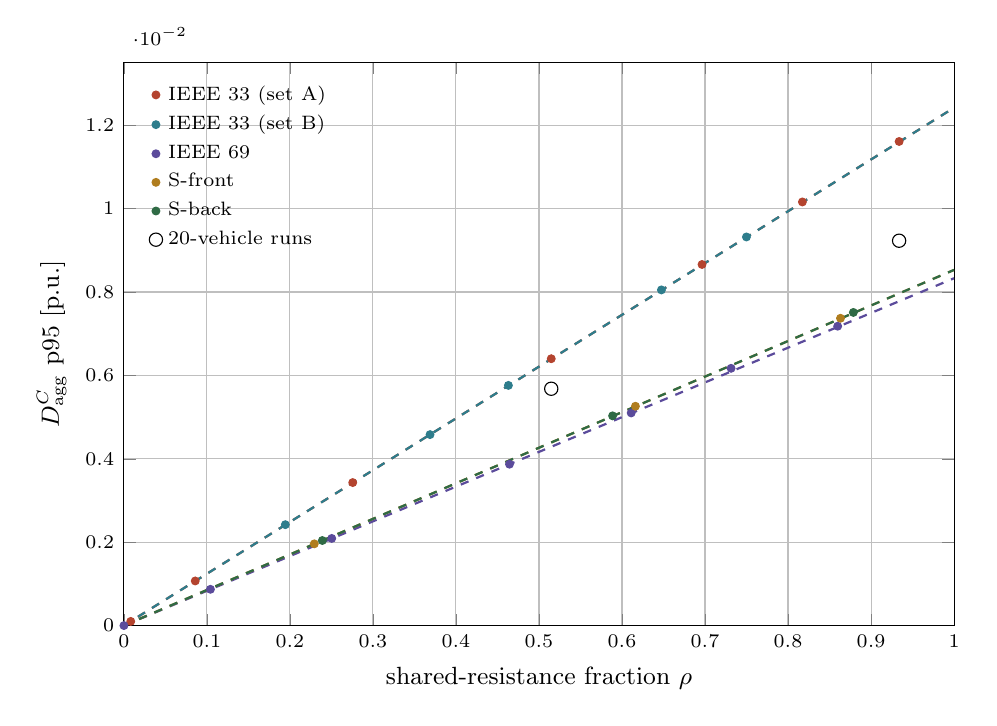
\begin{tikzpicture}
\begin{axis}[width=\columnwidth,height=0.72\columnwidth,
  xlabel={shared-resistance fraction $\rho$},
  ylabel={$D_{\mathrm{agg}}^{C}$ p95 [p.u.]},
  xmin=0,xmax=1,ymin=0,ymax=0.0135,grid=major,
  legend style={font=\scriptsize,at={(0.02,0.98)},anchor=north west,draw=none,fill=none},
  legend cell align=left,tick label style={font=\scriptsize},label style={font=\small}]
\addplot[c1,dashed,forget plot,thick] coordinates {(0,0) (1,0.01242)};
\addplot[c2,dashed,forget plot,thick] coordinates {(0,0) (1,0.01242)};
\addplot[c3,dashed,forget plot,thick] coordinates {(0,0) (1,0.00833)};
\addplot[c4,dashed,forget plot,thick] coordinates {(0,0) (1,0.00853)};
\addplot[c5,dashed,forget plot,thick] coordinates {(0,0) (1,0.00853)};
\addplot[c1,only marks,mark=*,mark size=1.4] coordinates {(0.0083,0.00010) (0.0860,0.00107) (0.2757,0.00343) (0.5148,0.00640) (0.6964,0.00866) (0.8173,0.01016) (0.9338,0.01161)};
\addlegendentry{IEEE 33 (set A)}
\addplot[c2,only marks,mark=*,mark size=1.4] coordinates {(0.1945,0.00242) (0.3688,0.00458) (0.4632,0.00576) (0.6475,0.00805) (0.7499,0.00932)};
\addlegendentry{IEEE 33 (set B)}
\addplot[c3,only marks,mark=*,mark size=1.4] coordinates {(0.0001,0.00000) (0.1043,0.00087) (0.2504,0.00209) (0.4645,0.00387) (0.6111,0.00510) (0.7314,0.00617) (0.8598,0.00718)};
\addlegendentry{IEEE 69}
\addplot[c4,only marks,mark=*,mark size=1.4] coordinates {(0.2294,0.00196) (0.6162,0.00526) (0.8632,0.00737)};
\addlegendentry{S-front}
\addplot[c5,only marks,mark=*,mark size=1.4] coordinates {(0.2391,0.00204) (0.5887,0.00503) (0.8787,0.00751)};
\addlegendentry{S-back}
\addplot[black,only marks,mark=o,mark size=2.4] coordinates {(0.5148,0.00568) (0.9338,0.00923)};
\addlegendentry{20-vehicle runs}
\end{axis}
\end{tikzpicture}

\caption{The hub's own drift term against $\rho$ on four topologies and 22
placements. Dashed lines are the closed form \eqref{eq:closedform}
---predictions, not fits; markers are measured 95th-percentile values. Each set
lies on its own line because $R_{mm}$ differs; no slope is a free parameter.
Circles mark the two 20-vehicle runs, the only points below their line.}
\label{fig:collapse}
\end{figure}

Four independent topologies and 22 placements agree with
\eqref{eq:closedform} to three significant figures. The one departure is
reported rather than removed: the two 20-vehicle runs fall \emph{below} the
line, dragging that set's fitted slope to $0.807$ of the closed form. A larger
fleet holds the hub nearer its cap for longer, so the bay switches less within
an interval; \eqref{eq:closedform} is an upper envelope in that regime rather
than an equality.

\subsection{Manipulation experiment}\label{sec:manip}
Correlation across two feeders is not a mechanism, so the structural hypothesis
was tested by construction. Two synthetic radial feeders were built differing
in exactly one property---whether the resistance of the hub's path is
concentrated near the substation (\emph{front-loaded}) or accumulates toward
the tip (\emph{back-loaded}, the long thin lateral shape)---with total path
resistance, hub layout, fleet, tariff and base-case minimum voltage ($0.9570$)
all held equal, and the same three-point $\rho$ sweep inside each arm
(Table~\ref{tab:manip}).

\begin{table}[!t]
\renewcommand{\arraystretch}{1.15}
\caption{Manipulation Experiment: One Structural Knob, Matched Base Voltage,
Identical $\rho$ Sweep Inside Each Arm. Band 0.005 p.u.}
\label{tab:manip}
\centering\footnotesize
\begin{tabular}{@{}llrrrr@{}}
\toprule
Arm & $\rho$ & Viol.\ min & slack p5 & $\Dagg^{C}$ p95 & $\Derr$ med\\
\midrule
\multirow{3}{*}{front-loaded}
 & 0.229 & 0  & 0.01204 & 0.00196 & 0.00135\\
 & 0.616 & 33 & 0.00988 & 0.00526 & 0.00136\\
 & 0.863 & 55 & 0.00847 & 0.00737 & 0.00138\\
\midrule
\multirow{3}{*}{back-loaded}
 & 0.239 & 0 & 0.01761 & 0.00204 & 0.00156\\
 & 0.589 & 0 & 0.01619 & 0.00503 & 0.00165\\
 & 0.879 & 0 & 0.01501 & 0.00751 & 0.00164\\
\bottomrule
\end{tabular}
\end{table}

The knob did not flip the mechanism: the drift term's slope against $\rho$ is
identical in both arms ($0.00854$, the closed form to three figures), and slack
falls with $\rho$ in both. What the knob controlled is the slack \emph{level}
---$0.0085$--$0.0120$ front-loaded against $0.0150$--$0.0176$ back-loaded at
the same base voltage---and that decides whether anything violates at all:
$0/33/55$ violating minutes against $0/0/0$, with the same fleet, the same
$\rho$ and the same drift. The supported causal structure is therefore
resistance profile $\rightarrow$ slack level $\rightarrow$ violation incidence,
separately from $\rho\rightarrow$ drift weight $\rightarrow\Dagg$, with the
second link exact and topology-independent. One confound is inherent and
stated: to reach the same base margin the two arms carry different total load
($0.415$ against $1.150$ of nominal), because a back-loaded profile drops less
voltage per kilowatt of load.

\subsection{One open question, narrowed}\label{sec:open}
Certified slack falls with $\rho$ on IEEE~33 ($-0.0080$, $-0.0120$) and in both
synthetic arms ($-0.0056$, $-0.0041$) but is flat on IEEE~69 ($+0.0007$);
Fig.~\ref{fig:split} shows both quantities. The manipulation experiment rules
out the resistance profile as the driver of that sign, since slack fell with
$\rho$ in both arms, and the invariance of $\gamma_C$ rules out any
fleet-drift explanation. What remains untested is the $\alpha$-fair
allocation's response on a feeder whose binding bus has a much longer upstream
path, and the interaction between hub placement and the load composition of the
other hubs. This is one sign of one derivative on one feeder; it does not
affect $\Lamt$, which uses the measured slack directly, and it is recorded as
open rather than resolved.

\begin{figure}[!t]\centering
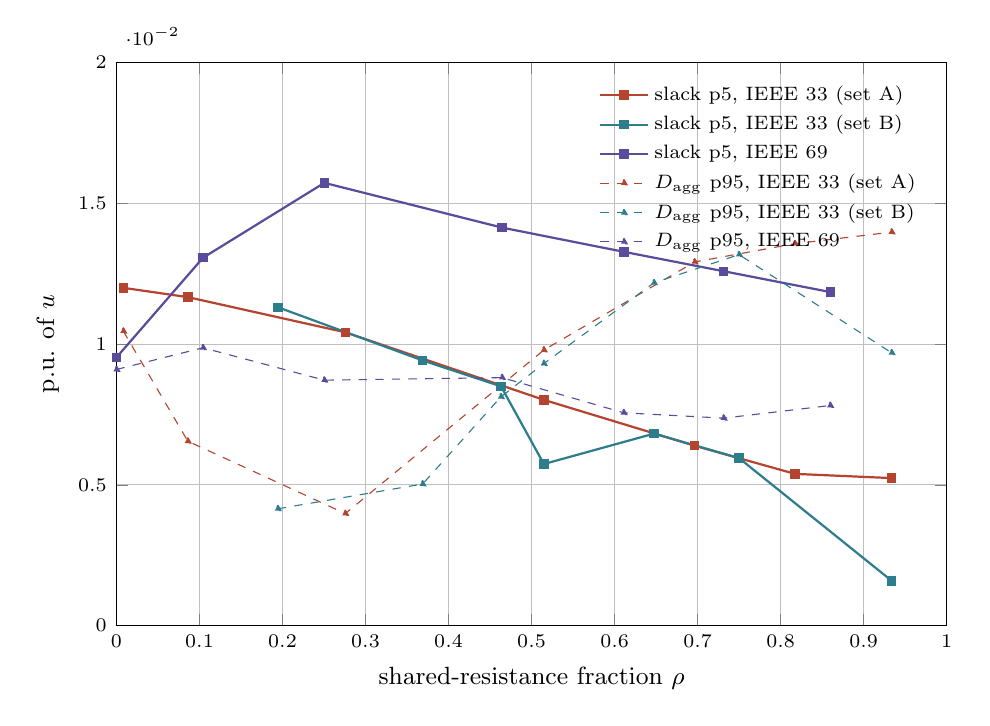
\begin{tikzpicture}
\begin{axis}[width=\columnwidth,height=0.72\columnwidth,
  xlabel={shared-resistance fraction $\rho$},
  ylabel={p.u. of $u$},
  xmin=0,xmax=1,ymin=0,ymax=0.02,grid=major,
  legend style={font=\scriptsize,at={(0.98,0.98)},anchor=north east,draw=none,fill=none},
  legend cell align=left,tick label style={font=\scriptsize},label style={font=\small}]
\addplot[c1,mark=square*,mark size=1.3,thick] coordinates {(0.0083,0.01200) (0.0860,0.01167) (0.2757,0.01042) (0.5148,0.00802) (0.6964,0.00639) (0.8173,0.00539) (0.9338,0.00524)};
\addlegendentry{slack p5, IEEE 33 (set A)}
\addplot[c2,mark=square*,mark size=1.3,thick] coordinates {(0.1945,0.01131) (0.3688,0.00942) (0.4632,0.00850) (0.5148,0.00574) (0.6475,0.00682) (0.7499,0.00595) (0.9338,0.00159)};
\addlegendentry{slack p5, IEEE 33 (set B)}
\addplot[c3,mark=square*,mark size=1.3,thick] coordinates {(0.0001,0.00953) (0.1043,0.01307) (0.2504,0.01573) (0.4645,0.01414) (0.6111,0.01328) (0.7314,0.01259) (0.8598,0.01185)};
\addlegendentry{slack p5, IEEE 69}
\addplot[c1,dashed,mark=triangle*,mark size=1.3] coordinates {(0.0083,0.01046) (0.0860,0.00655) (0.2757,0.00398) (0.5148,0.00979) (0.6964,0.01292) (0.8173,0.01357) (0.9338,0.01398)};
\addlegendentry{$D_{\mathrm{agg}}$ p95, IEEE 33 (set A)}
\addplot[c2,dashed,mark=triangle*,mark size=1.3] coordinates {(0.1945,0.00415) (0.3688,0.00503) (0.4632,0.00813) (0.5148,0.00931) (0.6475,0.01218) (0.7499,0.01318) (0.9338,0.00969)};
\addlegendentry{$D_{\mathrm{agg}}$ p95, IEEE 33 (set B)}
\addplot[c3,dashed,mark=triangle*,mark size=1.3] coordinates {(0.0001,0.00910) (0.1043,0.00987) (0.2504,0.00872) (0.4645,0.00881) (0.6111,0.00756) (0.7314,0.00737) (0.8598,0.00782)};
\addlegendentry{$D_{\mathrm{agg}}$ p95, IEEE 69}
\end{axis}
\end{tikzpicture}

\caption{Certified slack (solid, squares) and aggregate $\Dagg$ (dashed,
triangles) against $\rho$ on the three published-feeder sets. Slack falls with
coupling on IEEE 33 and is flat on IEEE 69; the aggregate $\Dagg$ behaves
inversely. Fig.~\ref{fig:collapse} shows that once the hub's own term is
isolated the two feeders agree exactly.}
\label{fig:split}
\end{figure}

\section{Generalisation Beyond Bus Fleets}\label{sec:disc}
Nothing in the derivation refers to buses. The criterion requires three things:
connection points that share feeder resistance ($\rho>0$), a load that can move
between them, and an allocation computed per site and refreshed on an interval.

\emph{Delivery-fleet depots} are the closest structural analogue, and the drift
term is larger: depot power steps as vehicles plug in and out, and depots
cluster on shared industrial laterals, so $\rho$ runs high. The mobility
constant is hours rather than minutes, which by Section~\ref{sec:tau} changes
$\gamma$ but not the form of the criterion.

\emph{Mobile and relocatable chargers} make $\rho$ a decision variable rather
than a network property: siting the unit chooses its shared resistance. Then
$\Lamt\le 1$ is a siting constraint, not a band-derating rule---and because
$\Dagg$ carries $\rho^{1}$, siting buys more than de-rating.

\emph{Vehicle-to-grid and shared building storage} make $\delta p$ signed,
which \eqref{eq:dagg} handles exactly since it is linear. Reverse flow can
raise voltage past the upper limit, so Theorem~\ref{thm:corner} must then be
applied at the upper corner as well as the lower.

The portable statement is the parameterisation: under per-site envelopes, a
fleet's grid impact is characterised by $(\rho,\ \mathrm{band},\ \max$
simultaneous draw, $\gamma,\ \Delta)$ and not by vehicle count, duty cycle or
dwell time except through those five.

\section{Threats to Validity}\label{sec:threats}
These are scope limits on what the evidence supports, not caveats on the
derivation.

\emph{(a) No measured feeder data.} Every closed-loop run applies synthetic
load, photovoltaic and tariff profiles to standard test systems. Nothing here
has been checked against metered distribution data, and real feeders carry load
volatility, unbalance and tap-changer action this model does not represent.
$\Dagg$ in particular is driven by intra-interval drift, exactly the quantity
real data would be most likely to change.

\emph{(b) One fleet model and one charger rating.} A single bus type, one route
structure, one timetable generator and one charging technology. $\gamma_C$ came
out invariant at $90$~kW, but that is $0.6\times$ the hub's single $150$~kW
bay: it is a charger property, and no run varied the bay rating or count, so
the slope of \eqref{eq:closedform} has been verified against topology but not
against $\gamma$.

\emph{(c) The operating threshold's generality is exactly what the holdout
tested.} Two radial feeders, two bands, one refresh cadence and the $\rho$
range of Section~\ref{sec:holdout}. The value $0.85$ carries no warrant outside
that box; $\Lamt>1$ is what should be used where it does not apply.

\emph{(d) The index does not cover one-at-a-time allocation.} For that
construction the index stays below unity while the AC solution violates,
because it fails for a separate and larger reason---factor-$N$
over-allocation---that neither error term models. The criterion is valid for
jointly certified envelopes and under-predicts otherwise.

\section{Conclusion}\label{sec:concl}
Per-site dynamic operating envelopes are secure in the model that produces
them, and this paper gives the condition under which that security survives in
the physical network when the flexible load is a mobile fleet sharing feeder
resistance. Two additive error terms are derived from the branch-flow
equations: an omitted-loss term, exact at $N$ hubs and convex in the allocated
caps, and a temporal-aggregation term that is first-order in intra-interval
drift. Their sum normalised by the certified slack gives one checkable
inequality, $\Lamt>1$ in \eqref{eq:lam}. That threshold is the general claim of
this work: it follows from the derivation, contains no fitted quantity, and
held with perfect precision and zero false positives across all 48 closed-loop
runs and both held-out published feeders. The relaxed trigger
$\Lamt>0.85$ is a secondary, operational recommendation only: it buys recall
inside the tested box of Section~\ref{sec:holdout} and, as
Section~\ref{sec:threats} states, carries no warrant outside it.

The empirical contribution is that the aggregation term is what makes envelope
failure a coupling phenomenon rather than a refresh-rate one, and that its
coupling dependence is entirely the network sensitivity weight: fleet drift
magnitude was invariant across every run, giving the closed form
\eqref{eq:closedform}, which matched measurement to three significant figures
on four topologies without a fitted quantity. A manipulation experiment
separated what controls violation incidence---the resistance profile, through
slack level---from what controls the mechanism---coupling, through the weight.
Future work should replace the synthetic profiles with measured feeder data,
vary the charger rating to test the closed form against $\gamma$ as well as
topology, and resolve the open sign reported in Section~\ref{sec:open}.

\section*{Reproducibility}
All simulation code, the topology generators, the parsed test-system data and
the result files behind every table and figure are available from the authors.
Every reported violation is produced by the AC solver at every simulated
minute, never by the linear model an allocation was optimised against.

\section*{Acknowledgment}
The authors would like to thank \dots

\bibliographystyle{IEEEtran}
\bibliography{refs}

\newpage

\begin{IEEEbiography}[{
\includegraphics[width=1in,height=1.25in,clip,keepaspectratio]{fig1}}]{Author One}
Biography text here.
\end{IEEEbiography}

\begin{IEEEbiographynophoto}{Author Two}
Biography text here.
\end{IEEEbiographynophoto}

\vfill

\end{document}
